\documentclass[11pt]{article}
\usepackage[margin=1in]{geometry}
\usepackage{amsmath,amssymb,booktabs,graphicx}
\usepackage[colorlinks=true,urlcolor=blue,citecolor=blue]{hyperref}
\title{When Does Correct Relational Geometry Support Unseen Composition?}
\author{Working draft: authors to be supplied}
\date{October 7, 2026: experimental scope closed}
\newcommand{\F}{\mathbb{F}}
\setlength{\emergencystretch}{3em}
\begin{document}
\maketitle
\begin{abstract}
We study when the correctness of specified mathematical relations contributes to unseen composition under matched output supervision. Permutation experiments identify a local compositional advantage, while initial joint affine finite-matrix and irreversible-polynomial protocols expose failures of intermediate-state inference and primitive generalization. A null-only-loss replacement does not restore the benefit. A final five-new-source matrix confirmation finds a 12.89 percentage-point activation-by-correctness interaction under a fixed budget. Transferring predicted readout-null components from correctly trained GELU operators improves linear composition by 8.75 points while preserving all first-step logits. Adequately optimized affine maps under the identical single-step loss recover most of the correctness benefit; the remaining relation-advantage interaction is 0.31 points with a descriptive interval crossing zero. We did not confirm an additional functional expressivity advantage. This study supplies known relations and operation order; it does not demonstrate spontaneous algebra discovery or a universal output-independent mechanism.
\end{abstract}

\section{Question and contribution}
Our question is whether the correctness of supplied relations contributes to held-out compositional prediction after controlling native and generator-output supervision. We distinguish detectable alignment, held-out representation prediction, and functional composition. These are separate endpoints. We use linear CKA \cite{kornblith2019} as an auxiliary alignment measure. CKA can change while functional behavior is largely preserved \cite{davari2022}; therefore accuracy and collision-pair performance are primary functional measures.

Group-structured latent representations and prediction of action sequences have already been demonstrated, for example by the Homomorphism AutoEncoder \cite{keurti2023}. Mechanistic analyses of finite-group composition also identify representation-theoretic circuits and test them by ablation \cite{chughtai2023}. Homomorphism-error probes predict synthetic language generalization by learning representation-level composition operators from expression pairs \cite{an2026}. Our intended contribution is a controlled correct-versus-matched-incorrect intervention, with identical correct output supervision, including conditions where a geometric relation has no measurable additional benefit. We train generator operators without compound representation targets, and evaluate their products separately. A complete related-work survey remains necessary before submission.

\section{Controlled intervention}
Let $h_\theta(x)$ be an encoder with fixed readout $W$, and let $T_A,T_B$ be two specified input operations. For the initial factorial experiments, learned affine row-vector operators are
\[
 R_A(h)=hM_A+b_A,\qquad R_B(h)=hM_B+b_B.
\]
The ordered word $AB$ always means first $T_A$, then $T_B$; its latent prediction is $R_B(R_A(h_\theta(x)))$. Compound inputs are used to construct evaluation truth but are never fed to the predictor. The program supplies the requested operation order, not the mathematical endpoint.

All four factorial conditions share correct native labels, native teacher logits, and correct generator-output distillation. Only the geometric correspondence changes. Within strata of length where relevant and the three visible gold answers, derangements $P_A,P_B$ preserve endpoint marginals. Both compositions of the discrete derangements are prohibited from returning an anchor to itself. This excludes discrete cancellation, not all possible numerical cancellation of learned operators.
\[
 L=L_{\mathrm{native\ CE}}+L_{\mathrm{native\ KD}}+L_{\mathrm{operator\ KD}}
 +\lambda\sum_{j\in\{A,B\}}\frac{\|R_j(h_\theta(x))-h_\theta(T_jP_jx)\|^2}{2s^2}.
\]
For correct pairings $P_j$ is the identity. A no-geometry condition uses $\lambda=0$ with the same input exposure and update count. The output-space diagnostic applies operators directly to full logits; it has fewer operator parameters and is not a capacity-matched causal control.

\section{Permutation results and error localization}
The primary permutation word is complement followed by inverse. The reversed word overlaps a visible statistic and is secondary. Six fitting repeats reuse three independently trained sources; they are not six independent source-model replications. The 20-epoch experiment continues the 10-epoch optimization state and is dependent on it.

\begin{table}[h]\centering
\begin{tabular}{lrr}\toprule
Geometric pairing & Collision accuracy(\%) & Pair double correctness(\%)\\\midrule
Both correct & 36.20 & 11.48\\
Complement correct only & 35.42 & 10.68\\
Inverse correct only & 30.92 & 5.68\\
Both matched incorrect & 29.87 & 4.30\\
No geometry, matched20epochs & 21.89 & 0.39\\\bottomrule
\end{tabular}
\caption{Same held-out20-epoch permutation collision test. Geometric correctness changes only hidden pairing; all conditions retain correct output supervision.}\end{table}
The correct group achieves36.20\% composition accuracy versus93.35\% with an oracle true intermediate. Repairing only first-step readout-nullspace error yields93.15\%, whereas repairing readout-row-span error yields59.09\%. These are diagnostic comparisons requiring the true intermediate, not deployable predictors.


\begin{figure}[h]\centering
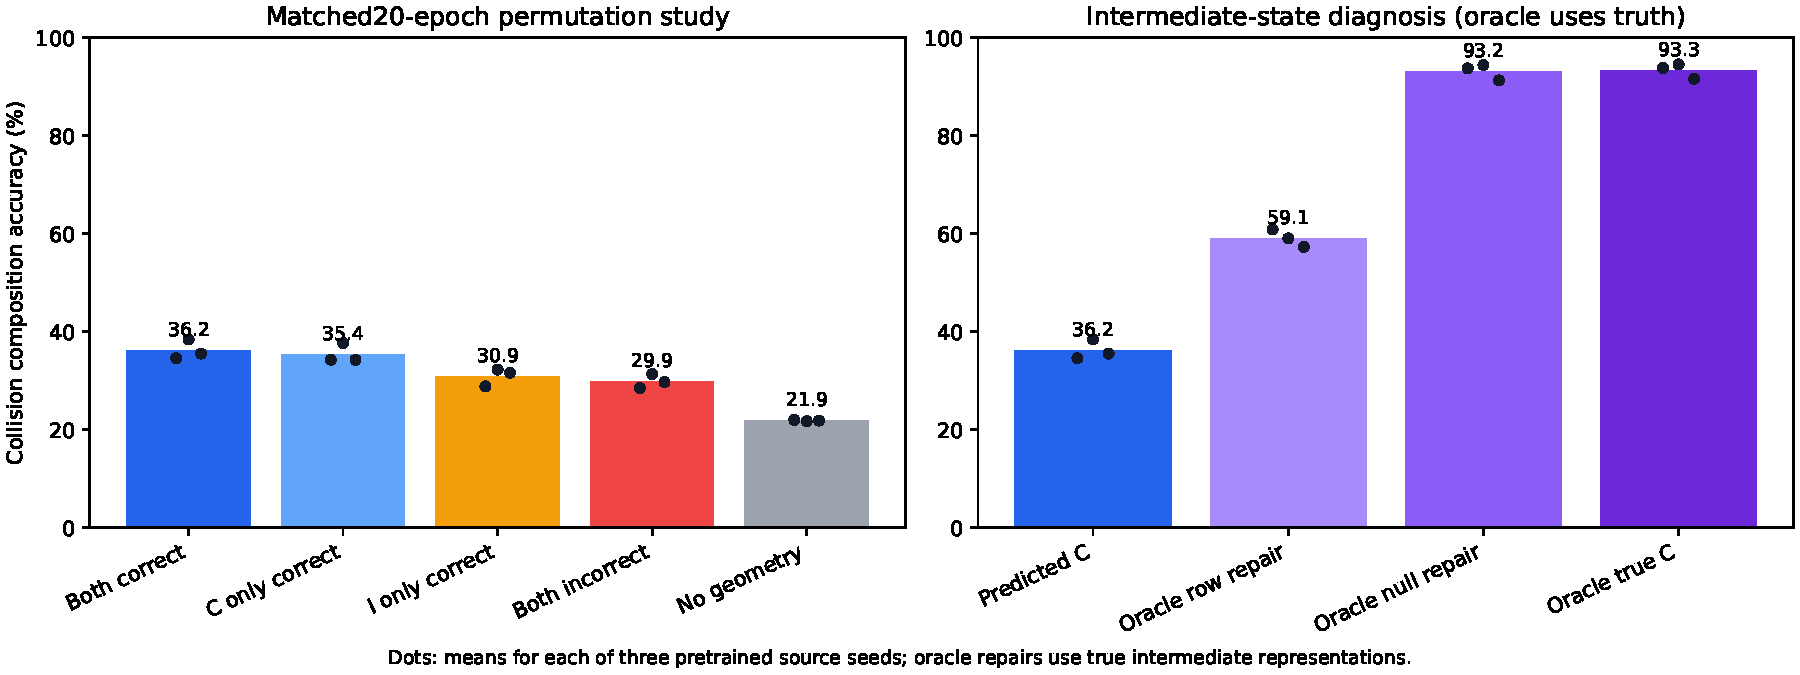
\includegraphics[width=\linewidth]{../results/algebra_relation_review/permworld_diagnostic.pdf}
\caption{Functional comparisons and oracle error localization. Oracle repairs require the true intermediate and are not predictions available at deployment.}
\end{figure}

Correct complement pairing accounts for most of the factorial advantage. The additional inverse-pairing increment is small with uncertainty crossing zero; we do not impose monotonicity as a success criterion. The matched 20-epoch no-geometry comparator was specified after the main 20-epoch outcomes were observed, using the previously fixed zero coefficient without tuning on those outcomes. Its timing must remain disclosed.

For a true intermediate $h_C$ and true endpoint $h_{CI}$, define $\delta_C=R_C(h)-h_C$. Then
\[
 R_I(R_C(h))-h_{CI}=\delta_CM_I+(R_I(h_C)-h_{CI}).
\]
The squared error includes the cross term between these two components. We report all terms rather than interpret their squared norms as additive causal fractions.
Let $P_W$ project onto the row span of the fixed numeric readout. Oracle repairs of $\delta_CP_W$ and $\delta_C(I-P_W)$ locate different intermediate errors. These repairs use the true intermediate and cannot count as inference. A nullspace repair preserves current linear numeric logits but need not remove nonlinear or other answer information. Its effect on subsequent predictions is evidence of fragility of the learned composition, not an output-independent mechanism.

\section{Two exact additional systems}
\paragraph{Finite matrix group.}
Inputs are invertible $2\times2$ matrices over $\F_{13}$, with task $\operatorname{tr}(X)$. Left actions use
\[
 A=\begin{pmatrix}0&1\\1&0\end{pmatrix},\qquad
 B=\begin{pmatrix}0&-1\\1&-1\end{pmatrix}.
\]
They generate a six-element noncommutative group with $A^2=B^3=e$ and $ABA=B^2$. Source, support, validation, and test partitions use disjoint complete group orbits. Visible answers are trace at $X,AX,BX$. The held-out ordered endpoint is $BAX$, with reverse order $ABX$ evaluated against the same primary target only where their gold answers differ.

\paragraph{Polynomials with an irreversible operation.}
Inputs are exact degree-three polynomials over $\F_{13}$. $T f(x)=f(x+1)$ and $D f=f'$. The native readout is evaluation at zero: visible answers are $f(0),f(1),f'(0)$ and the missing endpoint is $f'(1)$. Here $DT=TD$; this system cannot demonstrate order discrimination. Derivative-block and translation-orbit separation is audited for every actually observed and evaluated path. Complete semigroup closure cannot separate all inputs because $D^4f=0$. Polynomial collision pairs can connect derivative blocks, so their dependence is reported rather than treating every pair as an independent sample.

For illustration, $f(x)=x$ and $g(x)=x-x^2+x^3$ share visible answers $(0,1,1)$ but have missing answers $1$ and $2$. This algebra fixture is not itself a member of the formal exact-degree-three training distribution because $f$ has degree one.

\section{Prospective evaluation protocol}
The initial cross-domain protocol uses a common field size, four scalar input coordinates, a generic GELU encoder of width 128, three source seeds, six fitting repeats, and 900 fixed joint epochs. Later frozen-encoder confirmations use separately specified source counts, supports and budgets. No group or polynomial operations are hard-coded in the encoder. There are 1024 anchors per fitting pool, 512 source anchors, 128 validation anchors, 256 IID test examples, and 128 collision pairs. All six conditions receive five native state queries per anchor and identical forward-only supervision. The legacy permutation transformer uses bidirectional involution supervision and must be described separately.

The initial one-hot-plus-numeric encoder generalized native predictions but overfit generator prediction. A scalar encoder was selected using known matrix validation only, including a separately reserved confirmation set. This adaptation and pilot reuse are disclosed. No compound outcomes were used in that selection. A domain's compound test opens only after its known-only pilot reaches 95\% native and 90\% for both generators, and all 36 formal fits finish. Polynomial uses the matrix-selected scalar architecture without compound-based tuning.

Primary endpoints are ordered compound accuracy, collision-pair double correctness, and held-out representation prediction error normalized by actual displacement energy. CKA is auxiliary. All conditions' primitive scores and true-intermediate diagnostics are shown; failed primitive generalization limits interpretation. Source-cluster intervals describe three independently trained sources conditional on the fixed test set; six supports and overlapping polynomial blocks do not create extra independent sources.

\paragraph{Matrix.}
\begin{center}\begin{tabular}{lrr}\toprule Condition & Accuracy(\%) & Double correct(\%)\\\midrule
both correct & 9.44 & 0.52\\
a correct b wrong & 8.66 & 0.39\\
a wrong b correct & 7.94 & 0.26\\
both wrong & 8.92 & 0.39\\
no geometry & 7.55 & 0.26\\
output space & 7.23 & 0.26\\
\bottomrule\end{tabular}\end{center}
All 36 models have the same 900-epoch budget. Source-cluster uncertainty conditions on the shared test inputs. Output-space results are information diagnostics with fewer parameters.
Correct-vs-incorrect collision accuracy differs by0.52 percentage points; supplementary source-plus-whole-pair resampling gives[-1.56,2.73] percentage points. Thus a stable additional functional benefit is not established. Single-step scores are high, and true-intermediate prediction reaches99.22\%, whereas inferred composition reaches9.44\%.
\paragraph{Polynomial.}
\begin{center}\begin{tabular}{lrr}\toprule Condition & Accuracy(\%) & Double correct(\%)\\\midrule
both correct & 8.27 & 0.39\\
a correct b wrong & 8.20 & 0.52\\
a wrong b correct & 8.20 & 0.65\\
both wrong & 8.20 & 0.39\\
no geometry & 6.77 & 0.13\\
output space & 7.36 & 0.26\\
\bottomrule\end{tabular}\end{center}
All 36 models have the same 900-epoch budget. Source-cluster uncertainty conditions on the shared test inputs. Output-space results are information diagnostics with fewer parameters.
The all-source correct group reaches8.27\% versus8.20\% for incorrect geometry. Translation generator scores are91.80\%,87.11\%,87.50\% across sources; only the first meets the previously fixed90\% threshold. Its composition accuracy is7.42\%. Thus neither stable relation-specific benefit nor robust irreversible composition is established. Differentiation at the true intermediate achieves99.87\% overall.
The128 collision pairs connect39 derivative blocks into one connected component. They cannot be treated as128 independent block-level repetitions; source intervals condition on this fixed test set.


\section{Limitations and scope}
The initial joint affine matrix protocol has a small correct-minus-incorrect increment with an interval crossing zero; the subsequent frozen-encoder activation and convergence experiments are distinct interventions. Two polynomial sources miss the primitive translation threshold; their full outcomes remain in the primary report, with a known-only source stratum supplied separately. Even the passed source composes poorly. These findings identify limits of this affine-operator protocol and cannot refute every form of algebraic supervision. Generic geometric regularization greatly reduces displacement error relative to no geometry in both new domains, but wrong geometry often reduces it similarly and functional composition remains poor.

The three-gold-visible-answer collision ceiling applies only to a deterministic representation of those three answers. Full teacher probability distributions and hidden states can carry additional information. Pairwise double correctness above zero does not alone identify a relation-specific mechanism. The current study supplies relation supervision and composition rules, and cannot establish spontaneous discovery. Readout-nullspace analyses, output-space diagnostics, and correct-versus-wrong geometric comparisons answer different questions. Success in one domain does not establish a universal algebraic inductive bias.

\section{Margin-aware diagnostics and a directional-loss confirmation}

This follow-up was specified after the preceding experiments. Old-model diagnostics motivate a new-source, new-test intervention; they are not independent confirmation.

With row-vector conventions and first-step error $e$, the output change induced by its readout-nullspace part is $d_{\mathrm{null}}=eQ M_B W^\top$, where $Q$ projects onto $\ker W$. This preserves all first-step numeric logits, not every possible nonlinear answer code. We compare harmful rival-score shifts with the corresponding true-intermediate classification margins. Oracle-correct inputs are analyzed separately.

At equal perturbation norm (10\% of centered intermediate hidden RMS), old matrix-model collision accuracy falls from 99.2\% to 53.6\% in the actual null-error direction; the corresponding permutation figures are 93.3\% and 92.3\%. Random null directions are also tested at identical norm. The analysis is conditional on old trained models and test distributions and does not establish a universal domain ordering.

\begin{figure}[h]\centering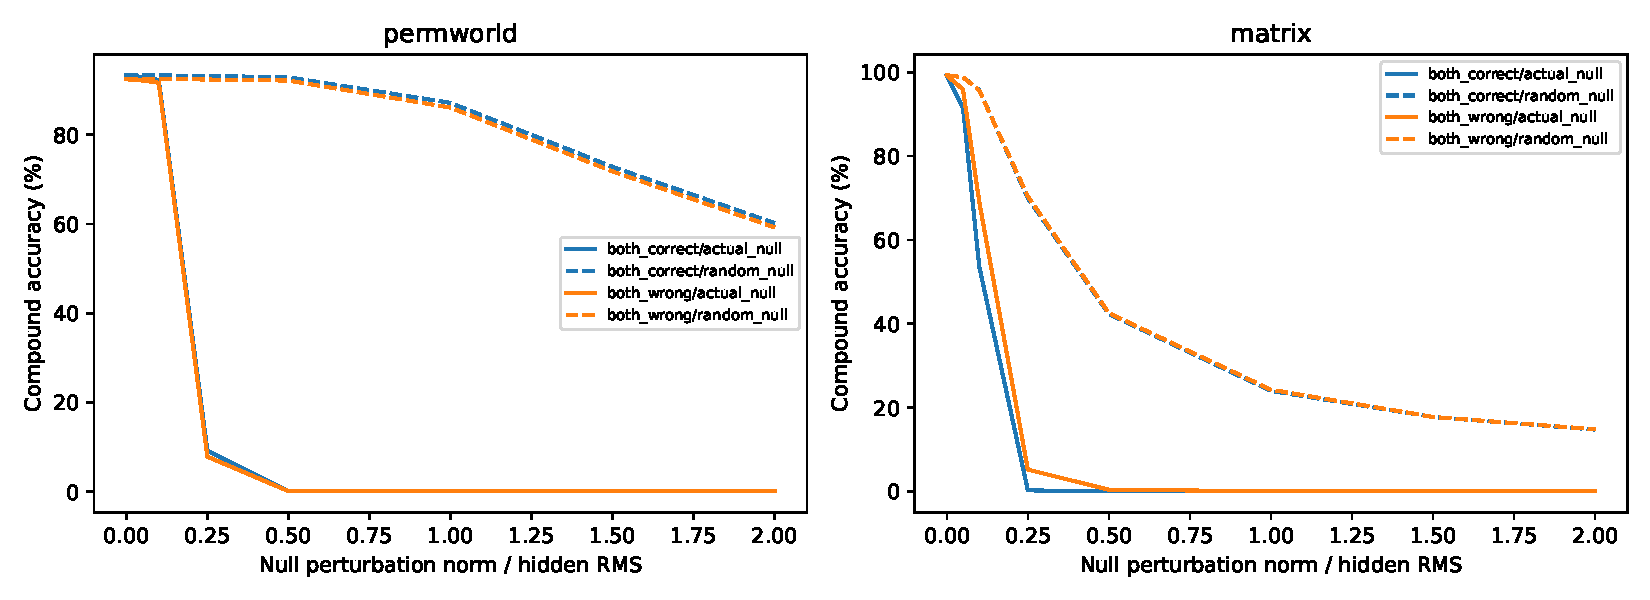
\includegraphics[width=\linewidth]{../results/downstream_harm_diagnostic_v2/perturbations.pdf}

\caption{Equal-norm actual-error and random-null perturbations of true intermediate states. Real intermediates are diagnostic information, not inputs available to the deployed predictor.}\end{figure}

\paragraph{Predictor capacity diagnostic.} We fit an affine residual and a one-hidden-layer GELU residual on only base-to-first-generator training states, using 2000 fixed updates and a frozen second operator and readout. Neither compound targets nor compound labels enter fitting. The nonlinear residual has approximately four times as many trainable parameters as the affine residual; this is not a capacity-matched comparison.

\begin{center}\begin{tabular}{llrr}\toprule Domain & First predictor & Compound (\%) & Both correct (\%)\\\midrule
matrix & Original affine & 9.64 & 0.00\\
matrix & Affine residual & 9.64 & 0.78\\
matrix & Nonlinear residual & 50.65 & 25.78\\
permworld & Original affine & 35.89 & 10.42\\
permworld & Affine residual & 38.75 & 13.18\\
permworld & Nonlinear residual & 45.62 & 20.05\\
\bottomrule\end{tabular}\end{center}

The capacity diagnostic uses three old source models per domain. Without matched-wrong nonlinear targets it cannot identify the causal effect of mathematical correctness. Identical-budget replay saves all predictors and forecasts and independently reproduces the initial diagnostic without tuning.

\paragraph{Prospective loss-direction intervention.} Each domain uses three new ordinary-source initializations and one fresh support pool per source. Full versus null-only geometric objectives are crossed with correct versus answer-matched wrong pairings. Each objective is normalized by the fixed ordinary teacher variance in its own space, using training states only. Native labels, teacher outputs, schedules, frozen readout, and all training budgets remain identical across the four arms. Permutation models train 20 epochs from initialization (distinct from the earlier dependent 10-to-20 continuation), and matrix models train 900 epochs. All twelve fits complete before the domain compound test opens.

Permutation sources reuse the original known-state corpus, so the new-source claim concerns initialization rather than new corpora. Their support and test orbits are excluded from all local archived input datasets. Matrix partitions are newly sampled, exclude previously examined matrix test orbits, and separate entire source/validation/support/test group orbits. Historical training orbits may recur under entirely new models.

\begin{center}\begin{tabular}{llrr}\toprule Domain & Direction/pairing & Compound (\%) & Both correct (\%)\\\midrule
matrix & full correct & 7.55 & 0.26\\
matrix & full wrong & 6.12 & 0.26\\
matrix & null correct & 9.64 & 0.78\\
matrix & null wrong & 9.51 & 0.78\\
permworld & full correct & 36.35 & 12.66\\
permworld & full wrong & 32.89 & 7.03\\
permworld & null correct & 12.55 & 0.21\\
permworld & null wrong & 14.66 & 0.42\\
\bottomrule\end{tabular}\end{center}

The predeclared primary statistic is the matrix accuracy interaction: $(\mathrm{null,correct}-\mathrm{null,wrong})-(\mathrm{full,correct}-\mathrm{full,wrong})$. Confidence intervals resample three source clusters and complete collision pairs. They do not treat the twelve models as twelve independent sources.

\begin{center}\begin{tabular}{lrr}\toprule Domain & Interaction (pp) & Source+pair 95\% interval\\\midrule
matrix & -1.30 & [-5.08, +2.60]\\
permworld & -5.57 & [-10.31, -1.46]\\
\bottomrule\end{tabular}\end{center}

Null-only loss removes the full-space row penalty as well as emphasizing null directions. In the new matrix study it lowers null error but permits larger readout-row state error; high primitive classification scores do not bound that error. Thus this experiment tests the specified replacement objective, not a scheme that retains the full-space term and adds null weighting.

No compound-outcome tuning or checkpoint selection was performed. A missing shared KD import was caught by a toy loss test and corrected before any permutation intervention fit; the initial script and pre-fit implementation amendment are retained. An initial diagnostic self-class division produced nonfinite margin statistics; the corrected implementation and independent rival-loop verification are preserved. The perturbation curves were unaffected.


\section{Final new-source mechanism confirmation}
An earlier three-source parameter-matched confirmation produced an activation-by-correctness interaction of 14.71 pp [9.51,20.05]. Posthoc predicted-null swaps and adequately fitted affine diagnostics on those same sources motivated the present hypotheses; a fresh-input check on reused sources is not new-source confirmation. We do not pool these exploratory and prior-confirmation outcomes with the final experiment.

We fixed this as the last experimental round before observing its new outcomes. Five previously unused source seeds (17291, 18401, 19507, 20611, 21713) were trained from scratch for 500 ordinary epochs and 900 correct single-generator preparation epochs. No old source checkpoint was reused. The five encoders, original maps and readouts were then frozen. Each source has its own 1024-anchor first-operator support, while the new source corpus and test are shared. Supports may overlap; source/validation/support/test complete group orbits are separated within the study. The new test excludes all 2688 previously examined matrix test orbits and contains 256 IID examples and 128 collision pairs. Historical inputs can recur in the new training partitions under new initialized models.

\paragraph{Matched activation and correspondence.}
Two-layer Identity and GELU first-operator residuals have identical width 256 and 65,920 trainable parameters, fixed original affine skip connections, matching initialization and zero final layers. Correct teacher logits, start states, schedules and 2000 AdamW updates are shared. Wrong geometry uses a complete derangement preserving all three visible gold answers. All four first-operator arms use zero weight decay, declared before fitting, to match the unregularized data objective of the convergence diagnostic. This harmonization differs from the earlier 0.0001-decay confirmation; the earlier results remain unchanged. The scalar encoder and source-preparation protocol are unchanged.

\paragraph{Predicted null-component transfer.}
For two predicted first states $\hat h_L,\hat h_G$ in the same source coordinates, with $P$ the row projector of the frozen full linear readout, we construct
\[
\hat h_{L\leftarrow G}=\hat h_L P+\hat h_G(I-P).
\]
The intervention uses no true intermediate state. It preserves every first-step logit, not only the winning class. Correct and matched-wrong GELU donors and reverse transfer are reported. Correct-null transfer yields +8.75 pp [+5.31,+12.42] improvement on collision AB; the correct-minus-wrong donor contrast is +8.44 pp [+4.92,+11.95]. Across interventions the maximum logit change is $2.23\times10^{-13}$. This tests a functional pathway in the specified frozen composition; hybrid states need not lie on the encoder manifold and the intervention does not remove all answer information.

\paragraph{Same-family, same-loss affine convergence.}
The two-layer Identity residual can express an unrestricted affine map. We solve exactly its shared empirical loss,
\[
 L(R)=\mathrm{KD}_{T=2}(R(h_0)W^\top+b_W,z_A)+0.25\,\frac{\|R(h_0)-h_A^{\mathrm{paired}}\|_F^2}{Nds^2},
\]
with $s^2$ fixed from correct training targets and the identical stored teacher logits $z_A$ used in all arms. There are no compound targets, ridge terms or validation-selected geometry weights. Float64 SVD whitening conditions the affine training design; readout-null coefficients have the exact least-squares solution, and readout-row coefficients are optimized by L-BFGS. Both OLS and original budget-linear row initializations are fixed in advance. The strongly convex quadratic term permits a gradient-based upper bound on remaining training-objective error. Independent analytic full gradients verify every solution. Both initializations, coefficient norms, condition numbers and float32-versus-float64 inference are retained. Changed parameterization, precision and additional budget are optimization diagnostics, not another equal-budget intervention.

\begin{table}[ht]\centering\small
\begin{tabular}{lrrr}\toprule First operator & Collision AB (\%) & Both correct (\%) & First-state NMSE\\\midrule
linear correct & 8.44 & 0.47 & 0.04647 \\
linear wrong & 9.45 & 0.31 & 0.06859 \\
nonlinear correct & 20.31 & 5.00 & 0.01973 \\
nonlinear wrong & 8.44 & 1.09 & 0.06874 \\
converged correct & 19.92 & 3.75 & 0.02963 \\
converged wrong & 8.36 & 0.31 & 0.08200 \\
\bottomrule\end{tabular}
\caption{Final five-source confirmation, with original budget-controlled arms and separately budgeted converged affine diagnostics. All predictions begin from the input representation and use the frozen second operator.}\end{table}

\paragraph{Predeclared contrasts.}
The same-budget activation-by-correctness interaction is +12.89 pp [+8.67,+17.03]. After affine convergence, the remaining GELU-versus-affine relation-advantage interaction is +0.31 pp [-5.86,+6.33]. Intervals resample five independent source clusters and the 128 common collision pairs; individual-source effects are provided in the experiment artifacts. These are descriptive intervals for separately stated hypotheses, not familywise-adjusted significance tests. Crossing zero cannot establish equivalence. All source gates and convergence checks are retained, without replacement of unfavorable sources.

\paragraph{Convergence and numerical qualification.}
The largest independently recomputed training-objective gap bound is $3.87\times10^{-12}$. Both fixed initializations yield identical compound classes, with a maximum predicted first-state difference of $6.55\times10^{-5}$. However, the affine design is ill-conditioned: condition numbers range from $8.65\times10^{7}$ to $1.29\times10^{8}$, and coefficient Frobenius norms range from $8.01\times10^{5}$ to $1.69\times10^{6}$. Replaying the complete affine--second-operator--readout pipeline in float32 changes 12/1280 correct-pairing and 43/1280 wrong-pairing collision predictions relative to float64. Aggregate correct/wrong accuracies are 19.92/8.36\% in float64 and 19.92/8.44\% in float32. Thus the main aggregate correctness advantage remains under this precision check, while individual predictions and high-norm coefficients are numerically sensitive. The convergence certificate concerns the finite empirical objective; it does not guarantee perturbation robustness or generalization to arbitrary inputs.

\begin{figure}[ht]\centering
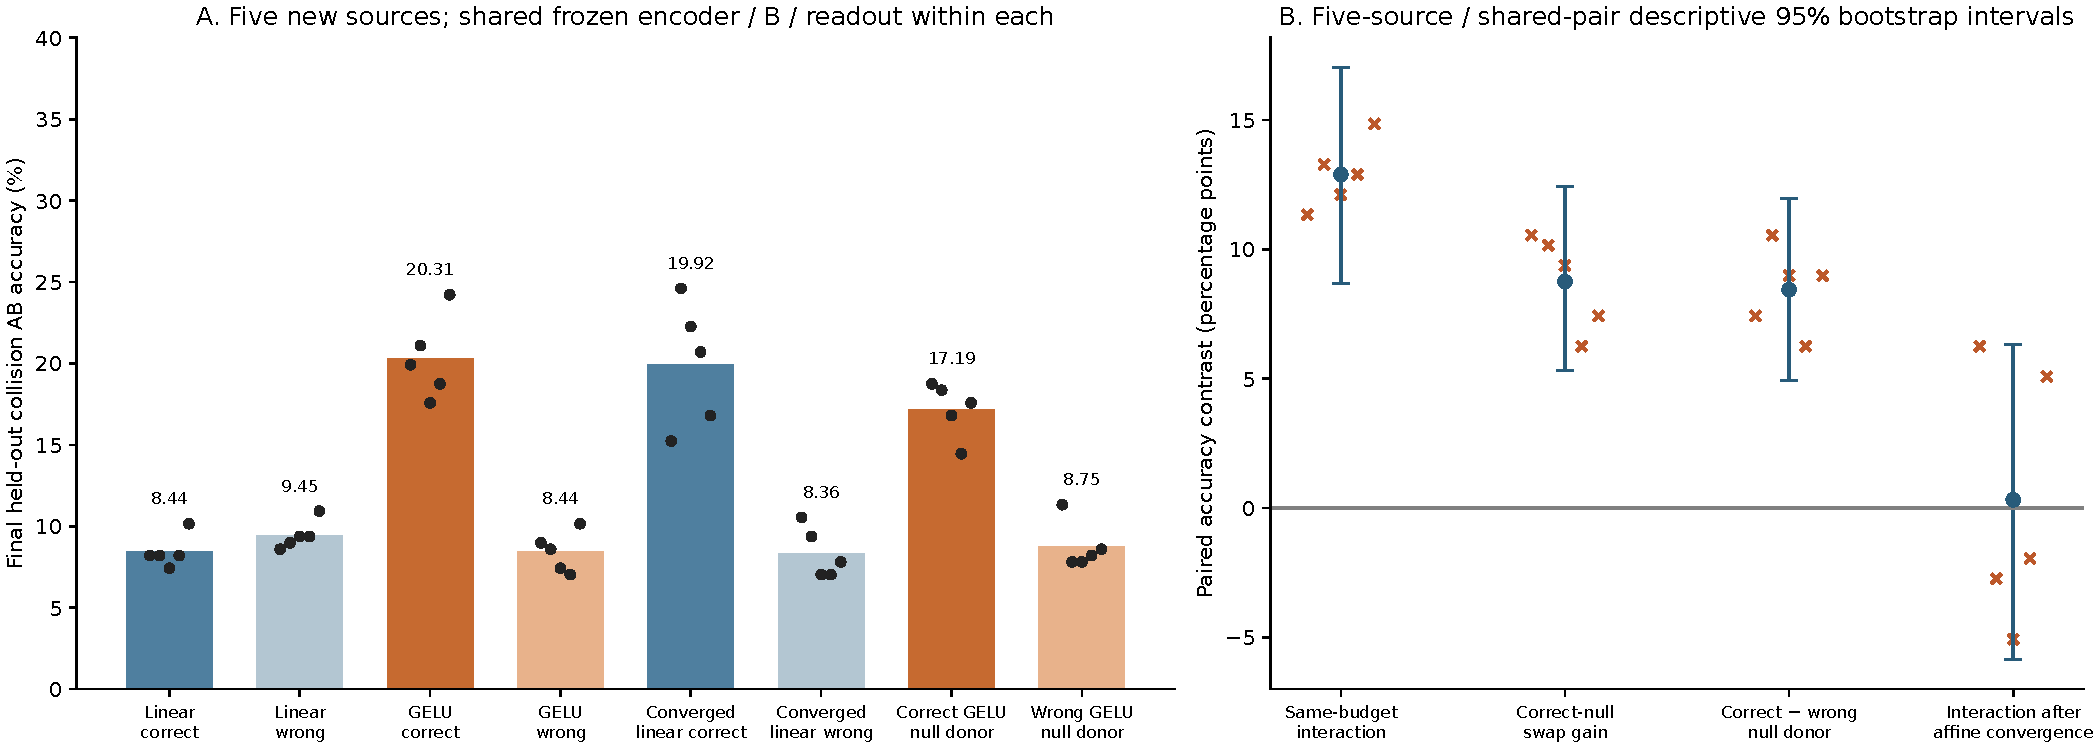
\includegraphics[width=\linewidth]{../results/final_mechanism_confirmation/final_confirmation.pdf}
\caption{Final confirmation with five new source initializations, predicted-component transfer, and the predeclared same-loss convergence diagnostic. Points show all five sources.}\end{figure}

\paragraph{Closing interpretation.}
We did not confirm an additional expressivity advantage in functional relation-specific composition after adequate affine fitting. State-fitting differences and unresolved numerical and optimization explanations are retained as limitations. We do not assign exact percentage contributions to optimization, numerical conditioning and expressivity. No additional domains, source seeds, losses or mechanistic training schemes are added after this fixed confirmation. The remaining work is manuscript refinement and submission preparation.


\bibliographystyle{plain}
\bibliography{references}
\end{document}
